\documentclass[a4paper,10pt]{article}
\usepackage{src/preamble}
\usepackage[
	backend=biber,
	maxalphanames=10,
]{biblatex}
\bibliography{accelerator.bib}


\begin{document}

\noindent
\begin{center}
	\textbf{{\Large RELAZIONE ACCELERATORE - IL CICLOTRONE}} \\
\end{center}

\noindent
\textbf{Autore: Alessandro Biagiotti} \hfill \textit{Università degli studi di Milano, Milano,
	Italia}
\\

\phantomsection
\makeatletter\def\@currentlabel{\texttt{(I)}}\makeatother
\label{sec:intro}
\noindent
\textbf{INTRODUZIONE:}
\\
Il ciclotrone fu il primo acceleratore ciclico inventato da Ernest Lawrence nel 1929-1930 e
successivamente patentato nel 1932, un esempio della struttura dell'acceleratore può essere vista
in Figura \ref{fig:cyclotron}. La particella, partendo da una posizione centrale, esegue un
moto spiraliforme verso l'esterno dell'acceleratore (aumentando quindi il raggio di curvatura a ogni
giro). L'acceleratore è costituito da due diverse \emph{dee}, un generatore a corrente alternata dà
un \emph{kick} alla particella ogni volta che questa si trova nel territorio di collegamento tra le
due dee. La dee all'interno della quale viaggia la particella non è altro che un conduttore che ha
le proprietà di un \emph{drift}.

\begin{figure}[h!]
	\centering

	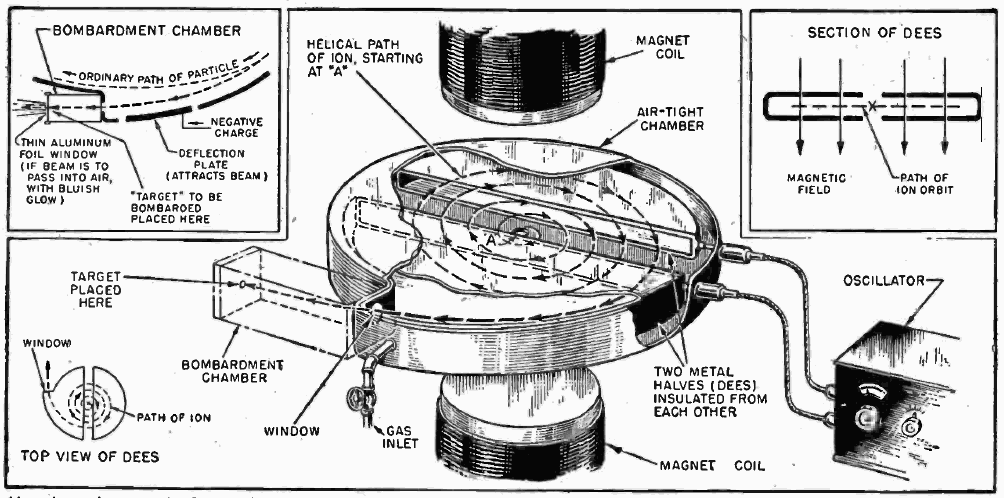
\includegraphics[scale=0.35]{fig/Cyclotron-diagram.png}
	\caption{
		La struttura di un ciclotrone
	}\label{fig:cyclotron}
\end{figure}

È chiaro come sia necessario che i periodi del generatore radiofrequenza e il periodo orbitale della
particella debbano coincidere, se così non fosse ci sarebbero dei problemi e la particella non
verrebbe accelerata in maniera efficace (o rischia di non venire accelerata proprio) \cite{bellomo}.

Nella prossima sezione andrò ad introdurre la fisica di questo acceleratore andando a spiegare le
conseguenze di alcune delle equazioni che si vedranno nel seguito, nella terza sezione andrò a
esporre alcune delle tecnologie che vengono correntemente utilizzate nel campo della fisica dei
ciclotroni.

\bigskip
\phantomsection
\makeatletter\def\@currentlabel{\texttt{(II)}}\makeatother
\label{sec:cyclotron}
\noindent
\textbf{ISOCRONIA DEL CICLOTRONE:}
\\
Il principio di funzionamento di questo modello di acceleratore è radicato nelle equazioni del moto
circolare. Se partiamo dalla seguente equazione che dichiara il modulo della forza agente su una
particella in moto all'interno di un campo magnetico
\begin{equation}
	F = q (E + v \times B)
\end{equation}
partendo da questa equazione, per il secondo principio della dinamica di Newton possiamo riscriverla
come:
\begin{equation}
	m a = q (E + v \times B) \label{eq:newt-lorentz}
\end{equation}
Se consideriamo la direzione centripeta possiamo rimuovere il campo elettrico dall'equazione in
quanto questo ha sola componente longitudinale (è responsabile per l'accelerazione della
particella). Inoltre ricordiamo l'equazione dell'accelerazione centripeta per il moto circolare
uniforme:
\begin{equation}
	m \frac{v^2}{r} = q v B
\end{equation}
Posso rimuovere anche il prodotto vettoriale dall'Equazione \ref{eq:newt-lorentz} perchè il campo
magnetico all'interno del ciclotrone è sempre perpendicolare alla direzione di spostamento (si può
notare anche dal modo in cui sono posizionati i magneti in Figura \ref{fig:cyclotron}). Facendo
alcune semplificazioni e ricordando la definizione di velocità angolare di un corpo in moto
circolare uniforme possiamo semplificare l'equazione precedente come segue:
\begin{equation}
	\omega = \frac{q}{m}B \label{eq:an-speed}
\end{equation}
Quest'equazione è probabilmente la più importante di tutto l'articolo poichè lega la velocità
angolare della particella alla carica (costante), al campo magnetico (che possiamo controllare e
quindi possiamo anche considerarlo costante) e alla massa, che per una particella all'interno di un
acceleratore che raggiunge velocità relativistiche è tutt'altro che costante. Questa dipendenza
della velocità angolare dalla massa viene ereditata dal periodo e questo significa che il periodo
d'orbita di una qualsiasi particella diminuisce man mano che la particella acquisisce massa una
volta giunti nella fase super-relativistica.

Il punto centrale è che Equazione \ref{eq:an-speed} dice che quando gli effetti relativistici
entrano in gioco l'acceleratore tende a perdere la condizione di isocronismo di cui si parlava
inizialmente, pertanto l'acceleratore non opera più come dovrebbe.

La soluzione banale per il problema sarebbe quella di fare in modo che il campo magnetico scali con
l'energia, e quindi scali con il raggio (siccome le due grandezze sono proporzionali, crescono di
pari passo) questo significherebbe che:
\begin{equation}
	B = B(r) \qquad \der{B}{r} > 0
\end{equation}
Ma ciò va poi a contraddire i requisiti minimi per la focalizzazione debole\footnote{L'indice di
	campo può essere riscritto come:
	\begin{equation}
		n = -\der{B}{r}\frac{r}{B}
	\end{equation}
	quindi questo va a legare la variazione del campo con la distanza dal centro e se l'indice di campo
	ha valore minore di $1$ allora questo ha comportamento ancora focalizzante.
}\cite{cyclotrons}. Per fare fronte a questo problema altre soluzioni sono state disegnate, come i
Sincrotroni e i Sincrociclotroni (che però esulano dagli obiettivi di questo documento), nel seguito
andrò a indicare alcune soluzioni che sono state proposte per l'isocronia del ciclotrone, rimanendo
nel campo dei ciclotroni, e senza perdite di focalizzazione.

\bigskip
\phantomsection
\makeatletter\def\@currentlabel{\texttt{(III)}}\makeatother
\label{sec:future-cyclotron}
\noindent
\textbf{SOLUZIONI AL PROBLEMA DELL'ISOCRONIA:}
\\

\clearpage

\printbibliography

\end{document}
